\documentclass[../../../patent_v1.tex]{subfiles}

\begin{document}

From abstract we can conclude speaker angles and sound intensities of individual 
speakers are very much important.

Speaker angles defines how the sound is gonna reach to the listener. Like is it 
reflecting from any surface or the sound source is directly pointed towards the listener.

Sound is nothing but oscillations of particles (typically air) in vibrational motion, which
transports energy through a medium.

\begin{figure}
    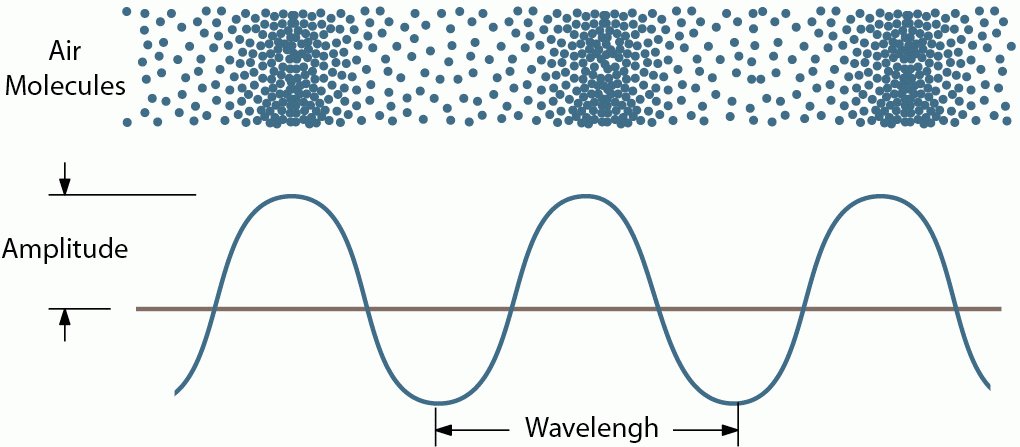
\includegraphics[width=\columnwidth]{sound_waves.png}
    \caption{Sound Waves}
\end{figure}

\FloatBarrier

Speakers push and pull surround air molecules in waves to generate a sound wave using a diaphragm.
Typically, this diaphragm is in conical shape hence it oscillates the molecules in the oval field. 

\begin{figure*}[ht]
    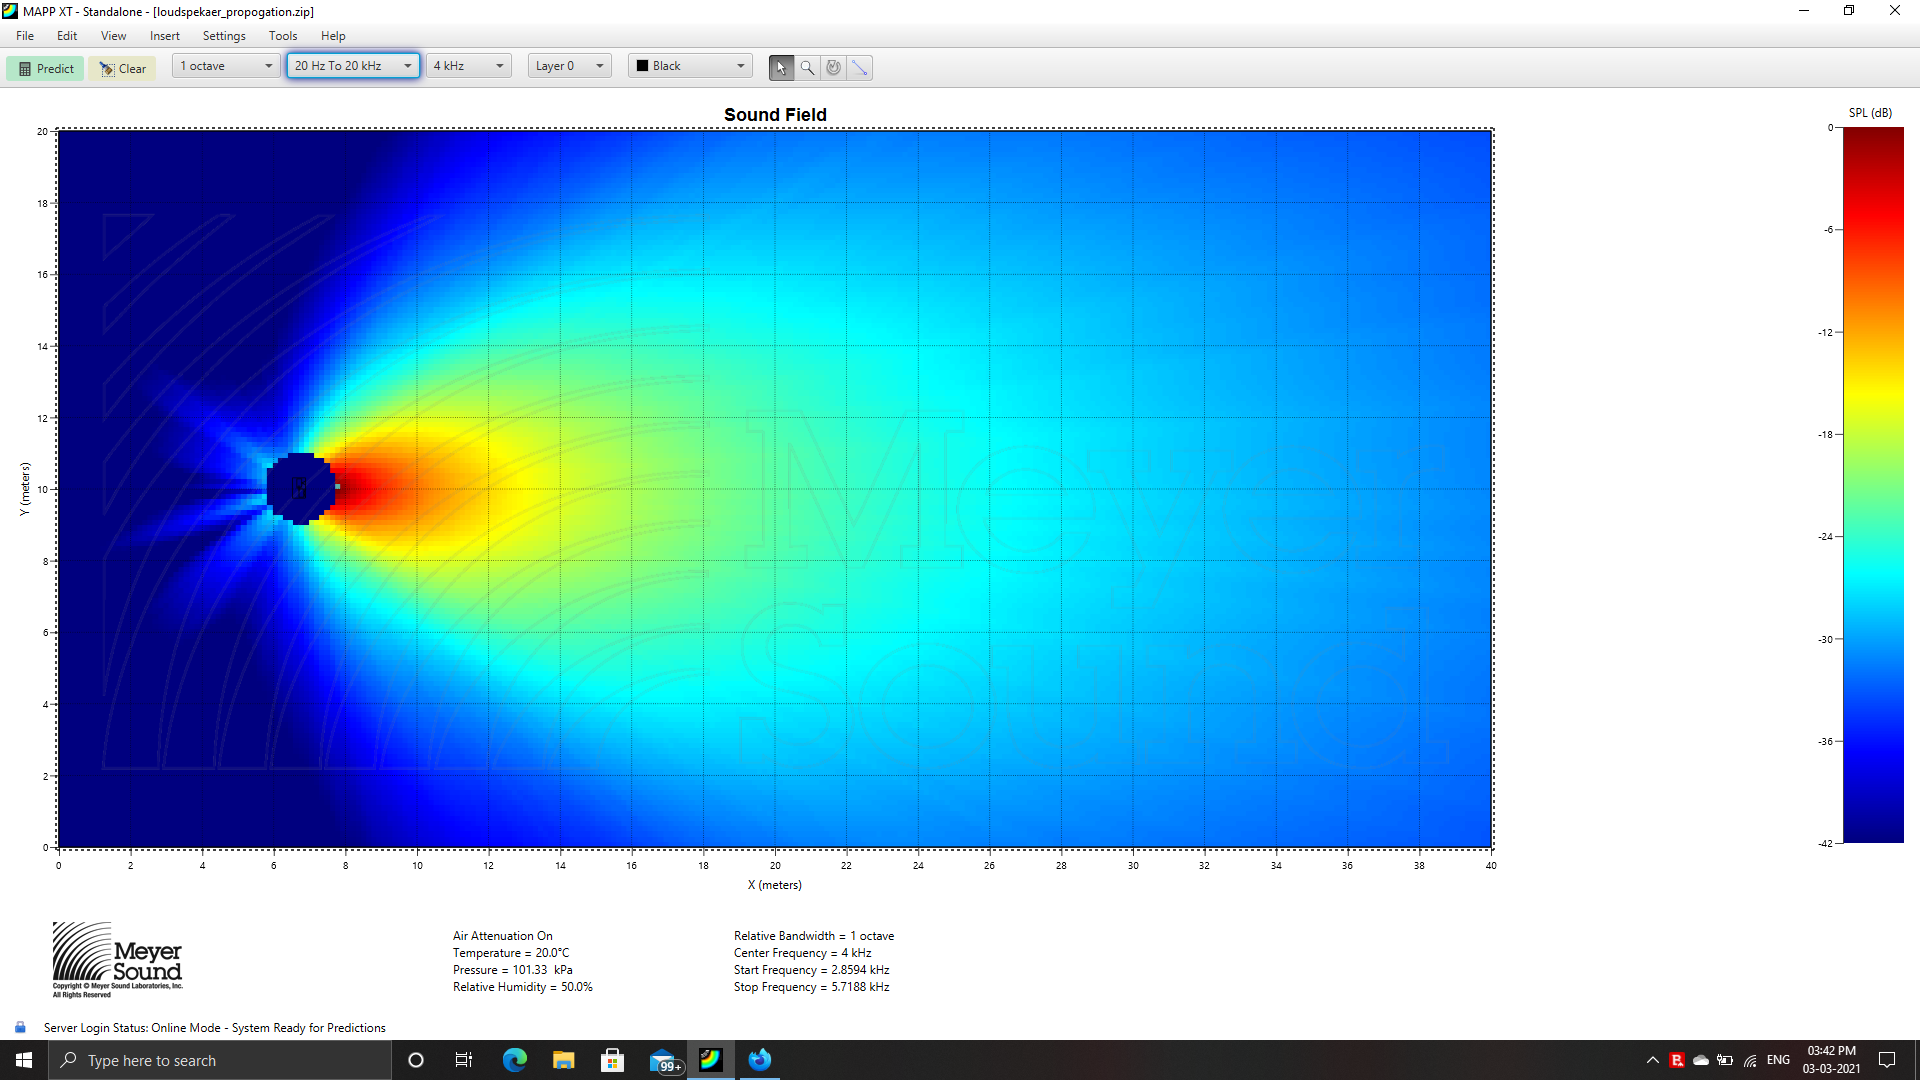
\includegraphics[width=1\textwidth]{sound_propogation_for_speaker.png}
    \caption{Sound propgation of speaker}
\end{figure*}

\FloatBarrier

Figure 3.2 shows the oval propgation of the sound field from the speaker. Where sound
intensity of speaker at some depth is denoted with heat map (dB). In front of the speaker
the sound intensity is maximum and it fades away as we go far away from the speaker. Where 
in the other hand it is much less at the back of the speaker. Since, it is oval in nature, 
the propogation to left and right is also less than that of front.

Figure 3.3 shows the reflection and reverberation of sound due to misalignment
and excessive sound intensity of speaker due to collision of sound waves onto walls. 
These reflections build up with each reflection and decay gradually as they are absorbed by the surfaces of Objects and walls
in the room. In this case, listener tends to hear direct sound and the repeated
reflected sound waves which might sound muddy and grabbled.

\begin{figure}
    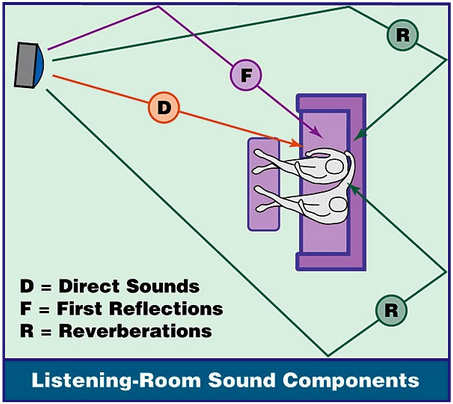
\includegraphics[width=\columnwidth]{reverberation.png}
    \caption{Reflection and reverberation of sound}
\end{figure}

\FloatBarrier

Hence, it becomes necessity to align the speakers as well as adjust the sound levels
in proper amounts to get best surround sound.

To overcome this scenario we experimented a five
block system. Which consists of,

\begin{description}
    \item[1.]Depth estimation unit (Cameras), to measure the depth of the listener
            from one reference point and feed these varibles to microporcessor for 
            further calculations.
    \item[2.]Microprocessor, to measure depth and calculate 
            panning and tilting angles as well as listener's depth
            from each speaker.
    \item[3.]Mechanical unit, to pan and tilt the speakers.
    \item[4.]Audio Processor Unit (Digitally controlled amplifier),
            to adjust the individual speaker gain using calculated 
            results from microporcessor.
    \item[5.]Speakers, to sound individual 4 channeled output.
\end{description} 

\end{document}